The permanent evolution in wireless technologies has shaped our lifestyle in ways not many could predict some few decades ago. Wireless communications are now an integral part of every aspect of our lives, from the way people communicate with each other, to being ubiquitous in our vehicles, our appliances and devices, and in the way people navigate land, sea or air, just to mention some examples \cite{wireless_applications}. Across the industry, companies are finding new and creative ways to employ these technologies. In agriculture smart sensors are being used to monitor crops and report information in real time \cite{sdr_sensors}. Mechanical devices can also use this same principle to monitor and obtain key information about vital processes and predict, for example, premature wear \cite{slip_rings}. Near field protocols in particular, such as Radio Frequency Identification (RFID), have completely changed some of our habits, enabling for example wireless payment solutions and eliminating the use of paper in credential validation systems, such as those used in public transportation.

These changes have been largely possible, due to breakthroughs in semiconductor manufacturing techniques, which have led to a dramatic plunge both in cost and size of integrated circuits, paving the way to a dramatic increase in the number of electronic devices available today \cite{semiconductors_evolution}. \autoref{fig:forecast_iot_devices} is a graph from a technical report by Strategy Analytics, predicting about 38 billion connected devices by 2025.

\begin{figure}[H]
  \centering
  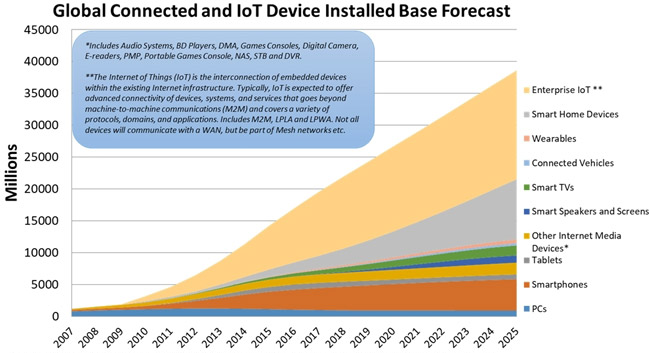
\includegraphics[width=0.75\textwidth]{forecast_iot_devices2}
  \caption{Strategy Analytics' forecast for the growth of IoT devices [Strategy Analytics]}
  \label{fig:forecast_iot_devices}
\end{figure}

Additionally, another key aspect in this new paradigm is the evolution of fibre optics technology which has resulted in the Internet backbone, allowing for the inter-connection of all these devices, fuelling our ever increasing demand for more data, re-shaping or creating entire markets such as online shopping or video on demand, and serving as the underlying infrastructure for mobile communication networks.

This momentum, however, comes with a new set of challenges. On one hand, having scores of electronic devices permanently active or even battery powered, requires us to come up with new ways to increase energy efficiency and develop disruptive battery technologies, if this reality is to become sustainable. On the other, the availability of more data, the sheer number of \emph{ad-hoc} connected nodes (the so called Internet of Things, IoT) and the mobile communications market in particular, have all called for vigorous new advances in the field of wireless protocols and architectures, sparking the interest both in academia and the industry. It is at the core of this ongoing revolution that software-defined radio (SDR) is making its mark.

%%%%%%%%%%%%%%%%%%%%%%%%%%%%%%%%%%%%%%%%%%%%%%%%%%%%%%%%%%%%%%%%%%%%%%%%%%%%%%%
\section{State of the Art}

The actual term \emph{software-defined radio} was coined by Joseph Mitola in a 1992 article entitled `Software radios - survey, critical evaluation and future directions' \cite{ntc92}, but some experiments have been conducted since the 70's, chiefly by military institutions in the United States (US) and Europe. Two early examples, the US Defence Advanced Research Projects Agency (DARPA) SpeakEasy project in 1991 and Joint Tactical Radio System (JTRS) in 1997 (shown in \autoref{fig:root_early_sdr_systems}), were both efforts to produce a unified radio system within the armed forces \cite{sdr_short_history}.

\begin{figure} [ht]
  \begin{subfigure}{.5\textwidth}
    \centering
    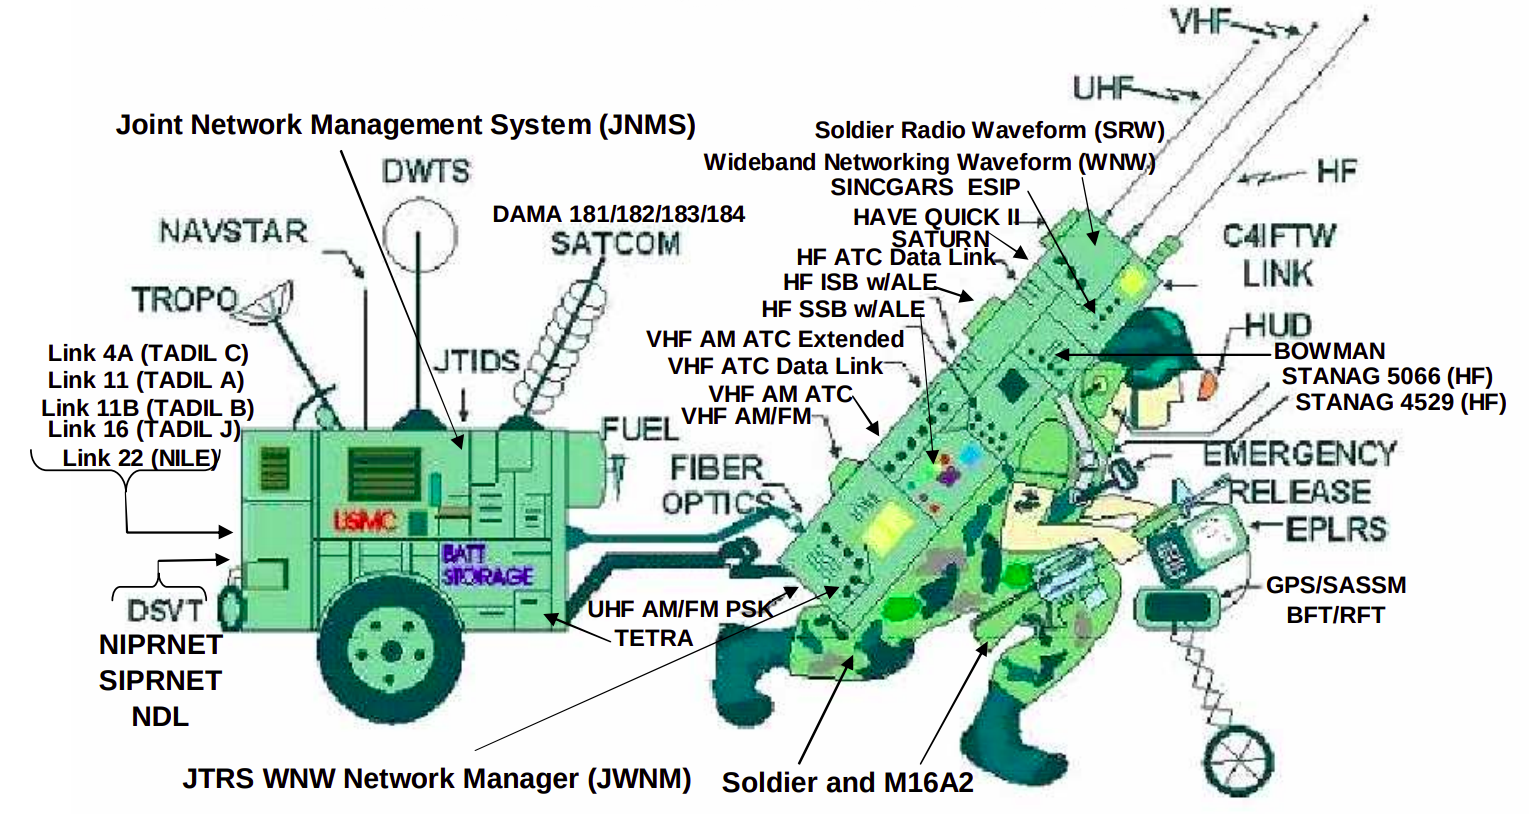
\includegraphics[width=.8\linewidth]{root_sdr_systems}
    \label{fig:root_sdr_systems}
  \end{subfigure}%
  \begin{subfigure}{.5\textwidth}
    \centering
    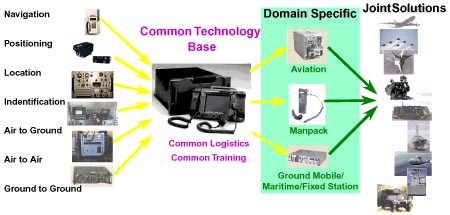
\includegraphics[width=.8\linewidth]{early_sdr_systems}
    \label{fig:early_sdr_systems}
  \end{subfigure}
  \caption[The JTRS multi-billion dollar program created by the US]{The JTRS was an ambitious multi-billion dollar program created by the US Department of Defence in 1997 to increase interoperability and waveform portability. It experienced difficulties, delays and  cost overruns leading to its cancellation in 2011. Despite that, it stimulated advances in SDR, both from manufacturers and other government agencies [\citeauthor{image:root_sdr_systems}].}
  \label{fig:root_early_sdr_systems}
\end{figure}

The increasing number of wireless protocols that have been developed nowadays however, such as Long Term Evolution (LTE) and beyond, for mobile communications; Zigbee, Bluetooth low energy (BLE) and Long Range (LoRa) for IoT; or new WiFi protocols for personal and machine-to-machine (M2M) communication, have brought the challenge to new levels. The need for a versatile transceiver design with the ability to handle several existing and future protocols, has never been bigger. In order to accomplish this task, one requires a flexible, re-configurable, and programmable framework. This is exactly the definition of SDR. A technology that is based on a software-defined approach, as opposed to hardware-based solutions. This means that features and functionalities, such as updating and upgrading through reprogramming, can be performed without having to replace the hardware on which they are implemented, opening the doors to the possibility of realizing multi-band and multi-functional wireless devices, effectively replacing hardware analogue blocks with software, and hardware description language (HDL) algorithms. Some examples of fields where SDR is being employed are:
\begin{itemize}
  \item Low-power IoT sensor nodes \cite{sdr_sensors}.
  \item Virtualized base stations controllers (BSCs) for mobile communication networks \cite{aict17}.
  \item Low-cost low earth orbit (LEO) satellite transceivers \cite{icssc16}.
  \item Academic research and educational tools, for example, in the fields of radio communications and digital signal processing (DSP) \cite{sdr_teaching}.
\end{itemize}

As far as SDR hardware is concerned, there are several options available today, ranging from low-end USB dongles with fairly limited RF and baseband performance, to high-end platforms which often include sophisticated signal correction hardware and algorithms, baseband computing power in the form of field-programmable gate arrays (FPGAs), and other advanced features, often bringing the price tag into the several thousands of US dollars.

There are quite a few key specifications to consider when characterizing the performance and capabilities of these platforms. A more incisive discussion into some of the possible SDR architectures, and their advantages and disadvantages, is presented in \autoref{chap:conceptual_overview}. As such, this section is limited to an overview of a few selected devices, representative of the spectrum of available options, focusing on some basic parameters, such as frequency range, bandwidth, sampling rate and resolution. These devices are the high-end professional level Universal Software Radio Peripheral (USRP) range from Ettus Research \cite{usrp_product_selector}, the open hardware and open source HackRF project from Great Scott Gadgets \cite{hackrf_one_product}, targeted at the academic/hobbyist audience, and the RTL-SDR \cite{rtlsdr_product}, an affordable Digital Video Broadcasting - Terrestrial (DVB-T) receiver with a RealTek chipset, that's been reverse-engineered by the community into a low-end SDR. A summary of the specifications for these devices, is laid out in \autoref{table:sdr_comparison}.

For the development of this thesis a HackRF One working as a transmitter, and an RTL-SDR as receiver, are used, and a more detailed description of these devices will be provided in \autoref{chap:demo_apps}.

\begin{table}[ht]
  \caption{Comparison of specifications from a few selected SDR platforms loosely spanning the spectrum of the currently available options}
  \label{table:sdr_comparison}
  \centering
  \begin{adjustbox}{width=1\textwidth}
  \begin{tabular}{>{\bfseries}l|c|c|c|c}
    \toprule
    \thead{Characteristics / Device} & \thead{USRP N210} & \thead{USRP B210} & \thead{HackRF One}  & \thead{RTL-SDR (RTL2832U)} \\
    \hline
    Full duplex                   & Yes                       & Yes                      & Half                    & No (only supports reception) \\
    Interface (throughput (Mbps)) & Gbit Ethernet (1000)      & USB 3.0 (5000)           & USB 3.0 (5000)          & USB 2.0 (480) \\
    MIMO                          & 2 TX - 2 RX               & 1 TX - 1 RX              & 1 TX - 1 RX             & 1 RX \\
    ADC/DAC resolution (bits)     & 14/16                     & 12/12                    & 8/8                     & 8 \\
    ADC/DAC sampling rate (Msps)  & 100/400                   & 61.4/61.4                & 20/20                   & 3.2 \\
    Frequency Range (GHz)         & 0-6                       & 0.07-6                   & 0.03-6                  & 0.024-1.776 \\
    Baseband hardware             & Spartan 3A-DSP 3400       & Spartan 6                & XC6SLX75                & CPLD \& 8051 + demod \\
    Cost [USD]                    & \multicolumn{1}{c|}{1750} & \multicolumn{1}{c|}{690} & \multicolumn{1}{c|}{10} & \multicolumn{1}{c}{300}
  \end{tabular}
  \end{adjustbox}
\end{table}

As far as SDR software is concerned, there are also quite a few alternatives available. Hardware developers tend to provide driver libraries that allow low-level interaction such as configuration, diagnostics, firmware upgrade and basic tx/rx (\emph{libhackrf} for the HackRF or \emph{librtlsdr} for the RTL-SDR, for example), and on top of that, SDR development frameworks have emerged. Two well-known frameworks are the PothosSDR project \cite{pothossdr_project} (which also includes the SoapySDR library \cite{soapysdr_project}) and the GNU Radio (GR) project \cite{gnuradio_project}. Since most of the projects are open source, the connections between them tend to assume more of a mesh layout than being completely separate. Further above these frameworks, sit SDR client programs that allow for a more high-level experience, such as GQRX (an SDR receiver powered by GNU Radio and the Qt graphical toolkit) and CubicSDR (an SDR receiver based on the SoapySDR platform). \autoref{fig:sdr_frameworks} is a block diagram loosely depicting some of the mentioned SDR libraries and client programs.

\begin{figure}[ht]
  \centering
  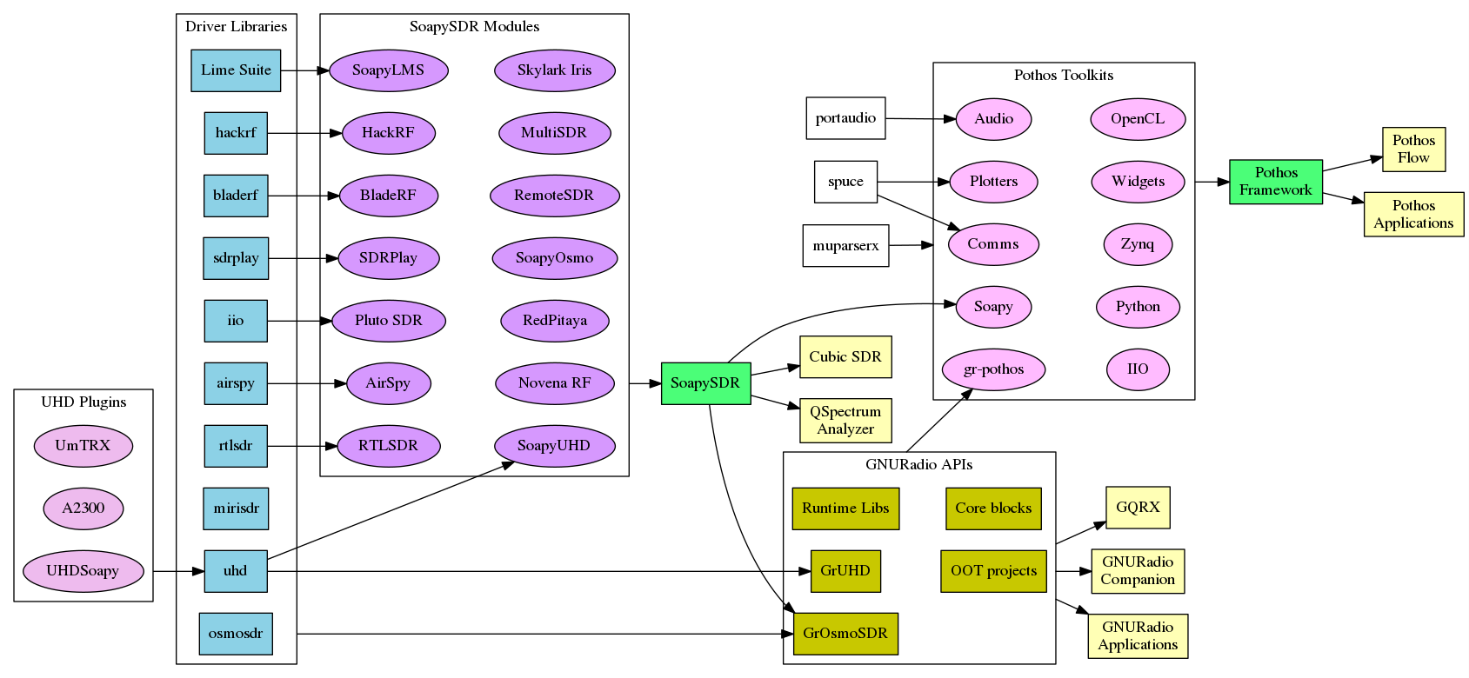
\includegraphics[width=\textwidth]{sdr_frameworks}
  \caption{Some of the most widely used SDR platforms and their inter-connections [\citeauthor{pothossdr_project}]}
  \label{fig:sdr_frameworks}
\end{figure}

A noteworthy exception is SDR\# (SDR Sharp), a modular client which depends only on low-level hardware libraries and not on any SDR framework, and can be seen in \autoref{fig:sdr_sharp}.

\begin{figure}[ht]
  \centering
  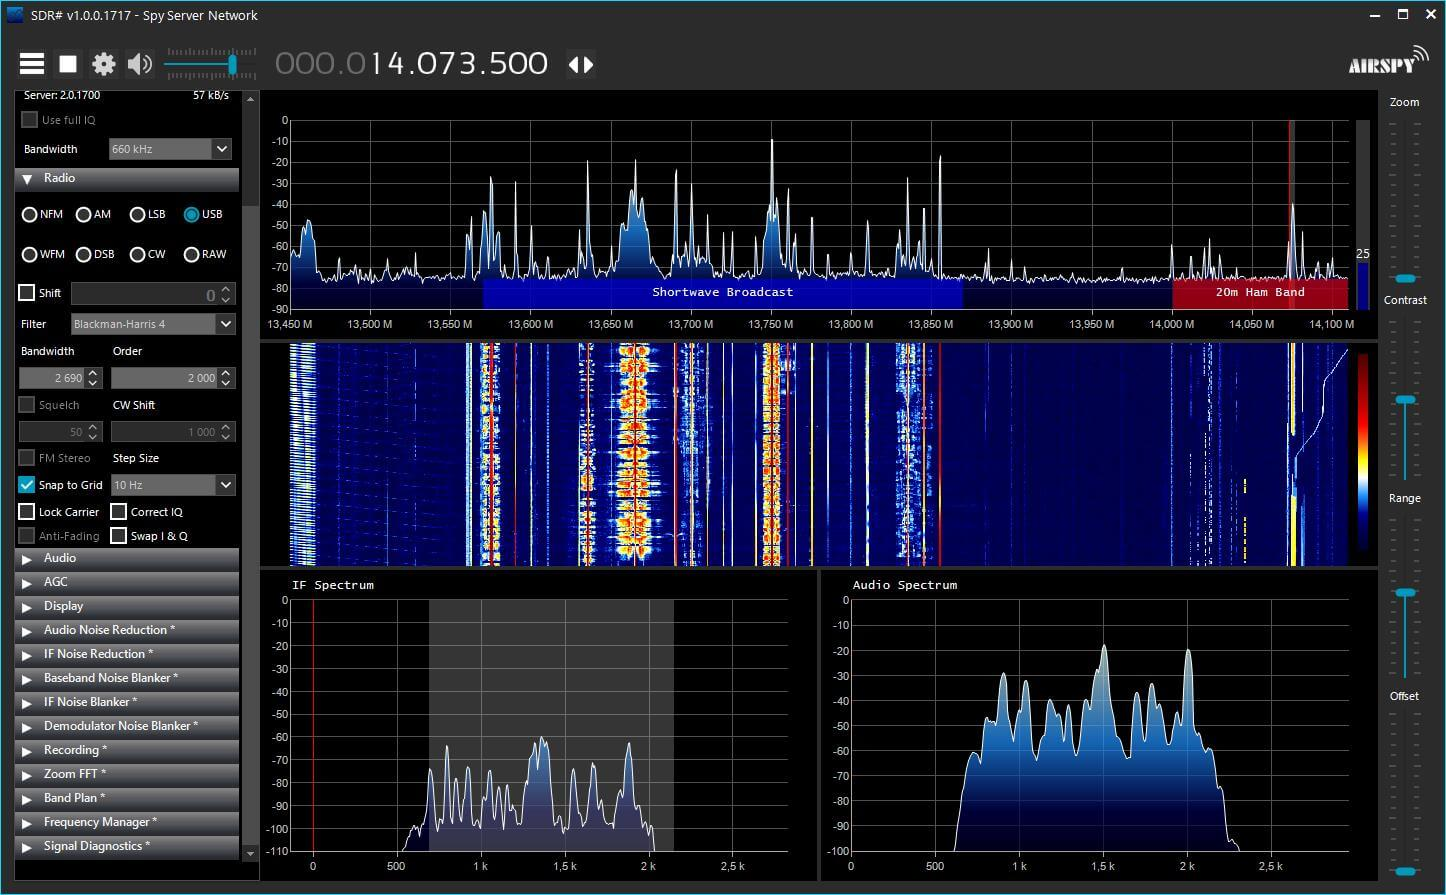
\includegraphics[width=0.85\textwidth]{sdr_sharp}
  \caption[SDR\# a popular SDR client]{SDR\# a popular SDR client developed in C\# by Airspy, who are also hardware SDR device manufacturers [\citeauthor{image:sdr_sharp_image}]}
  \label{fig:sdr_sharp}
\end{figure}

There is also some support within proprietary packages, such as MATLAB that provides wrappers for the USRP and RTL-SDR devices.

Finally, it is also common to encounter pure Python libraries for SDR research and experimentation. These can be simple packages that wrap low-level hardware libraries (such as \emph{pyrtlsdr} which is a Python wrapper of \emph{librtlsdr}), and which are often used in conjunction with other signal processing libraries such as \emph{NumPy} and \emph{SciPy}. Other types of libraries also exist that focus, not so much on the hardware interaction, but on SDR/DSP algorithms implementation (the \emph{komm} library \cite{komm_project} and the \emph{scikit-dsp-comm} library \cite{scikit-dsp-comm_project}, are good examples).

Of the mentioned frameworks, GNU Radio is very mature, flexible and exhaustive. An impressive amount of different technologies have been implemented, or at least prototyped, in it, such as Global System for Mobile Communications (GSM) \cite{gr-gsm} and Long-Term Evolution (LTE) \cite{gr-lte} receivers; several satellite technologies such as LEO and geosynchronous orbit (GEO) weather satellite demodulators \cite{meteor_m2_decoding}, and Cubesat receivers \cite{icssc16}; phase alternating line (PAL) and National Television System Committee (NTSC) decoders \cite{pal_decoder} \cite{ntsc_decoder}; 802.11a/g/p WiFi and 802.15.4 Zigbee transceivers \cite{wime_project}, frequency modulation (FM) transceivers \cite{gnuradio_wbfm_receiver}, among many others. For this reason, it has been chosen to implement the demonstration applications in this thesis. A more detailed description of the GNU Radio SDR framework is presented in \autoref{chap:demo_apps}.

%%%%%%%%%%%%%%%%%%%%%%%%%%%%%%%%%%%%%%%%%%%%%%%%%%%%%%%%%%%%%%%%%%%%%%%%%%%%%%%
\section{Objectives}
\label{sect:objectives}
The main objective of this thesis is to create a software framework of DSP algorithms that can demonstrate the potential applications of SDR as an educational tool for digital communication systems, in the academic context.

This will be achieved, first by creating a library that includes implementations of several key algorithms relevant to signal processing in the context of telecommunications, such as digital modulators, FIR interpolators/decimators, channel models and impairments (for example, an additive white gaussian noise (AWGN) channel model, phase/frequency offset, IQ imbalance and DC offset), frequency and phase correction techniques, clock synchronization, forward error correction (FEC) algorithms, among others. The library will be developed in Python, which provides a good balance between speed of development and performance. It also makes it easy to re-use in other environments, such as GNU Radio (GR), which natively support Python. This framework will constitute the backbone of the project and can, in the future, be extended with other algorithm implementations, as learning exercises for fellow students/users in DSP subjects. Several key best practices will be used (such as unit testing framework and code documentation) so as to introduce users to the importance of these requirements in a software project lifecycle, in order to keep a fairly high standard of code quality and documentation.

The library will also be accompanied by a set of \emph{Jupyter notebooks}, that will be created to demonstrate the workings and usage of the developed modules. This is aimed at, not only showing the concepts, but also highlighting the benefits of the Jupyter framework for rapid prototyping and proof of concept demonstrations.

On top of this library, and as means of direct application demonstration, two GNU Radio applications will be developed. The first is a \emph{wideband frequency modulation} (WBFM) demodulator, optimized for embedded systems (GR already includes a WBFM implementation \cite{gnuradio_wbfm_receiver} and a brief comparison with the proposed algorithm will be presented). The main idea is to demonstrate how SDR applications have the potential to replace legacy analogue systems with relative ease. The second application will be a \emph{phase-shift keying} (PSK) transceiver. This will also be developed in GR, but instead of implementing the algorithms directly in GR blocks, it will make full use of the Python library and simply create thin wrappers in GR. Requisites for this PSK transceiver include BPSK and QPSK modulations, channel impairments corrections, and both propagated and radiated real-time environment functionality with actual hardware deployment (as opposed to only performing offline file processing in simulation environment).

%%%%%%%%%%%%%%%%%%%%%%%%%%%%%%%%%%%%%%%%%%%%%%%%%%%%%%%%%%%%%%%%%%%%%%%%%%%%%%%
\section{Thesis Structure}

This thesis is organized in five chapters.

\autoref{chap:introduction} provides a brief overview of the evolution of wireless communication systems, with a focus on the reasons leading to the large increase of connected devices in recent years. It then introduces the concept of SDR systems with a brief historical background, and discusses in more detail the state of the art, with respect to both hardware and software solutions.

\autoref{chap:conceptual_overview} presents a theoretical description of a few of the most commmon SDR architectures. An initial introduction defines the main blocks in an SDR system (radio frequency (RF) section, intermediate frequency (IF) section and signal processing section), and then a more detailed discussion of each section is presented. In each of them, the general aspects of each architecture along with their advantages and disadvantages, and main applications are discussed. In order to better understand the implications of each architecture, it's important to be aware of key RF concepts and parameters which are widely used to evaluate the dynamic performance of SDR systems (and RF communication systems in general). Towards this end, an initial section on these topics is presented, prior to discussing the SDR architectures.

\autoref{chap:sksdr_lib} describes the algorithms developed for the DSP/SDR library (the library is named SKSDR after \emph{science kit SDR}). This library constitutes the backbone of the project and is later used for SDR demonstration applications. Each algorithm is discussed in detail in a separate section. In addition to the detailed theoretical explanation, a summary of the API is also provided, as well as usage examples, both using IPython (Python REPL interpreter) and Jupyter notebooks.

\autoref{chap:demo_apps} is dedicated to the SDR demonstration applications. An initial section describes, in more detail, the hardware used and the GNU Radio platform, giving some examples of simple GR flowgraphs. \autoref{sect:WBFM_Receiver_with_alternate_algorithm} starts by describing the specifications of a typical FM broadcast system. It then describes the standard WBFM demodulation implementation in GR and proceeds to explain in depth, the alternative proposed algorithm. There are many techniques for FM demodulation but they generally fall within a set of 4 classes of algorithms. These are identified and briefly described, and both the GR standard implementation and the alternative implementation are framed within them. After this, the PSK transceiver is also presented in detail in \autoref{sect:psk_transceiver} with both the GR flowgraphs design and execution being demonstrated, together with some result analysis.

Finally \autoref{chap:conclusions} concludes the thesis, including a discussion on achieved results, key takeaways and future work.
